\documentclass{article}
\usepackage[spanish]{babel}
\usepackage{amsmath}
\usepackage{amsthm}
\usepackage{amsfonts}
\usepackage{amssymb}
\usepackage[utf8]{inputenc}
\usepackage{graphicx}
\usepackage{multicol}


\begin{document}


\section*{Hoja de ejercicios \\ Agentes y búsqueda}
\noindent
Inteligencia Artificial \\
Facultad de Ciencias, UNAM\\
Pérez Jacome David.

\vspace{15pt}

\noindent
\small{
\begin{enumerate}
\item Llenar la siguiente tabla con base a los tipos de entorno que le corresponda a cada tarea:
    \begin{table}[!h]
        \small
        \centering
        \begin{tabular}{|p{1.7cm} | c | c | c | c | c | c|} \hline
            \textbf{Entorno} & \textbf{Observable?} & \textbf{Agente?} & \textbf{Determinista?} & \textbf{Episódico?} & \textbf{Estático?} & \textbf{Discreto?} \\ \hline
            Go & Totalmente & Multiagente & Estratégico & Secuencial & Dinámico & Discreto \\ \hline
            Traducción automática & Totalmente & Individual & Determinista & Episódico & Dinámico & Continuo \\ \hline
            Voz-a-texto & Completamente & Multiagente & Estocástico  & Episódico & Dinámico & Continuo \\ \hline
            Clasificación de objetos en imágenes & Totalmente & Multiagente & Determinista & Episódico & Semidinámico & Continuo \\ \hline
            Aumento de calidad de video & Parcialmente & Individual & Determinista & Secuencial & Semidinámico & Continuo \\ \hline
        \end{tabular}
    \end{table}
    \item Considerar el mundo de la aspiradora con 3 cuartos (casillas) configurados de la siguiente forma:
    
    \begin{center}
            \begin{tabular}{|c|c|} \hline
                (A, 1) & (B, 1) \\ \hline
                (C, 1) & - \\ \hline
            \end{tabular}
    \end{center}
    Es decir, sólo están disponibles los cuartos A, B y C. El 1 indica sucio y el 0 limpio. Suponiendo que el agente comienza en el cuarto A, con todos los cuartos sucios y el objetivo es limpiar todos los cuartos, formalizar analíticamente el problema como un problema de búsqueda asumiendo un costo $c(s_i, a, s_j)=1$ para cualesquiera estados $s_i, s_j$ y cualquier posible acción $a$. 
    \item A partir del problema anterior, dibujar la gráfica de búsqueda del problema y proponer una solución óptima.
    \item Considerar el siguiente problema de búsqueda con \textbf{inicial} $s_0$ y  final $s_6$:
    \begin{center}
        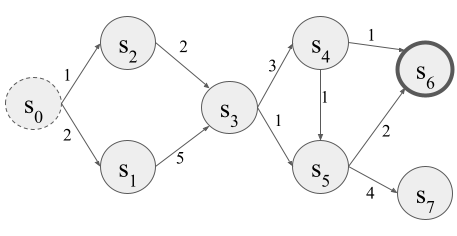
\includegraphics[scale=0.5]{images/SearchExercise.png}
    \end{center}
    Describir a partir de la gráfica el problema en forma analítica.
    \item A partir del problema anterior, utilizar el algoritmo de \textbf{depth-first search} para encontrar el árbol de búsqueda y la solución.
    \item A partir del problema 2, utilizar el algoritmo de \textbf{best-first search} para encontrar el árbol de búsqueda y la solución, usar función de costo del problema.
    \item A partir del problema 2 y la siguiente función heurística de abajo,
    \begin{table}[!h]
        \centering
        \begin{tabular}{c | c c c c c c c c} \hline
             ~ & $s_0$ & $s_1$ & $s_2$ & $s_3$ & $s_4$ & $s_5$ & $s_6$ & $s_7$ \\ \hline
             $\mathbf{h}$ & 4 & 3 & 3 & 2 & 1 & 1 & 0 & $\infty$ \\ \hline
        \end{tabular}
    \end{table}
    obtener el árbol de búsqueda y la solución por medio del algoritmo de \textbf{Greedy Best-First Search}.
    \item A partir del problema 2 y de la heurística anterior usar el algoritmo $\mathbf{A^*}$ para obtener la solución y el árbol de búsqueda.
    \item A partir del siguiente problema de búsqueda (inicial: $s_0$, final: $s_6$):
    \begin{center}
        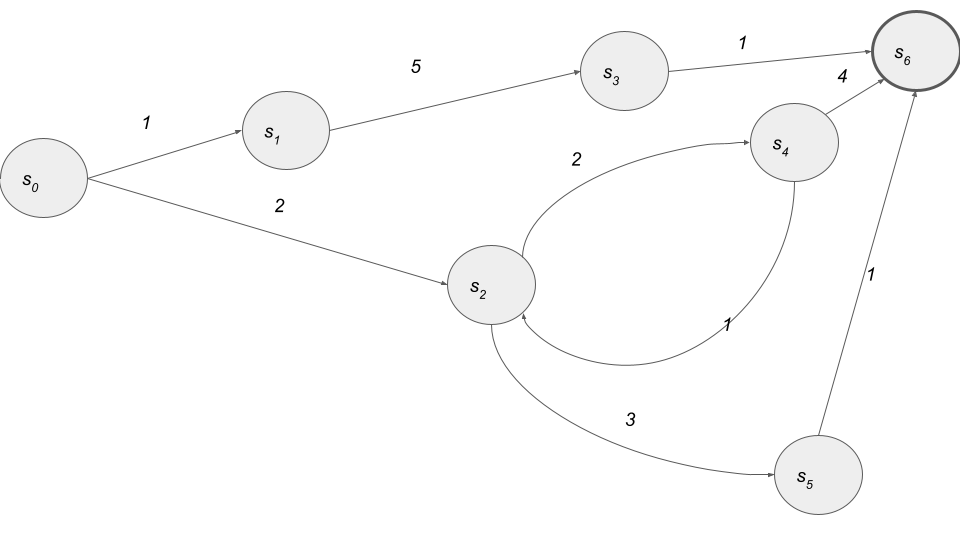
\includegraphics[scale=0.28]{images/space.png}
    \end{center}
    aplicar el algoritmo de \textbf{primero mejor} (Best-first search), dibujar el árbol de búsqueda, y dar la solución resultante. 
    \item A partir del problema de búsqueda anterior y usando la siguiente heurística:
    \begin{table}[!h]
        \centering
        \begin{tabular}{|c | c c c c c c c|} \hline
            ~ &  $\mathbf{s_0}$ &  $\mathbf{s_1}$ &  $\mathbf{s_2}$ &  $\mathbf{s_3}$ &  $\mathbf{s_4}$ &  $\mathbf{s_5}$ &  $\mathbf{s_6}$ \\ \hline
            $\mathbf{h}$ & 3 & 2 & 6 & 1 & 2 & 1 & 0 \\ \hline
        \end{tabular}
    \end{table}
    Aplicar el algoritmo de $\mathbf{A^*}$, dibujar el árbol de búsqueda y dar la solución encontrada.
\end{enumerate}

\end{document}
